\chapter{Konzept}

\label{AppendixKonzept}

\section{Zweck des Dokuments}\label{KonzeptZweck}

Das Konzept dient als Anleitung für die Realisierungsphase. Die in der Konzept
erarbeiteten Details müssen in der Realisierung eingehalten un umgesetzt
werden.

\subsection{Teilkonzepte}

Durch die in der Studie gewonnenen Erkentnissen, werden in der Phase Konzept
verschiedene Teilkonzepte erstellt.

Im Teilkonzept «Portalname» wird der Name des Produktes erarbeitet.

Im Teilkonzept «Design- und Bedienkonzept» werden die Ansichten der Applikation
in Mockups umgesetzt. Es werden die Benutzer Use-Cases vom Besucher sowie der
Konzert-Erfasser aufgezeigt.

Im Teilkonzept «Softwarekonzept» werden die Datenflüsse hinter den Mockups
aufgezeigt, sowie die Datenbankstruktur aufgebaut.

Im Teilkonzept «Testkonzept» werden die einzelnen Systemtests aufgelistet sowie
ausgearbeitet wie granular welche Teile der Software getestet werden sollen.

Im letzten Teil des Konzept-Dokuments wird im Fazit dokumentiert, wie und warum
das Konzept von den vorhergehenden Phasen des Projekts abweicht.


\clearpage
\section{Portalname}\label{portalname}

Der Portalname wurde in einer Brainstorming-Session von Damian Senn auf
den Namen \textbf{«Gigpillar»} festgelegt. Der Name ist angelehnt an die Werbepfeiler in
Städten, wo oft Werbeplakate für Konzerte hängen.

Die folgenden Ideen wurden in Betracht gezogen, jedoch war keine Domain mehr
verfügbar oder der Name überzeugte nicht:

\begin{itemize}
  \item{} upto.com («What are you up to?»)
  \item{} up-to.com
  \item{} uptoin.com
  \item{} gigup.com
  \item{} gigsta.com («Gigs to attend»)
  \item{} gigin.com
  \item{} gigsin.com
  \item{} gixin.com («Gigs in»)
  \item{} dualact.com («Loud act»)
  \item{} trecnoc.com («Concert» rückwärts)
\end{itemize}

\clearpage
\section{Design- und Bedienkonzept}\label{design--und-bedienkonzept}

\subsection{Mockups}

\subsubsection{Homepage}

Die Homepage ist die erste Seite, die der Besucher sieht, wenn er/sie die
Applikation direkt über \href{https://gigpillar.com/}{gigpillar.com} aufruft.
Auf den ersten Blick ist die Suche sowie ein grosses Bild (Banner) eines Gigs
zu erblicken. Weiter sind Links zu gängigen Funktionalitäten wie Gig hinzufügen
sowie das Login in einer Navigation erreichbar.

Unter dem Banner werden Gigs in nächster nähe des Besuchers aufgelistet, der
Link «change location» führt weiter zur Suchresultate Seite um den
entsprechenden Filter anzupassen.

\begin{figure}[!htb]
  \centering
  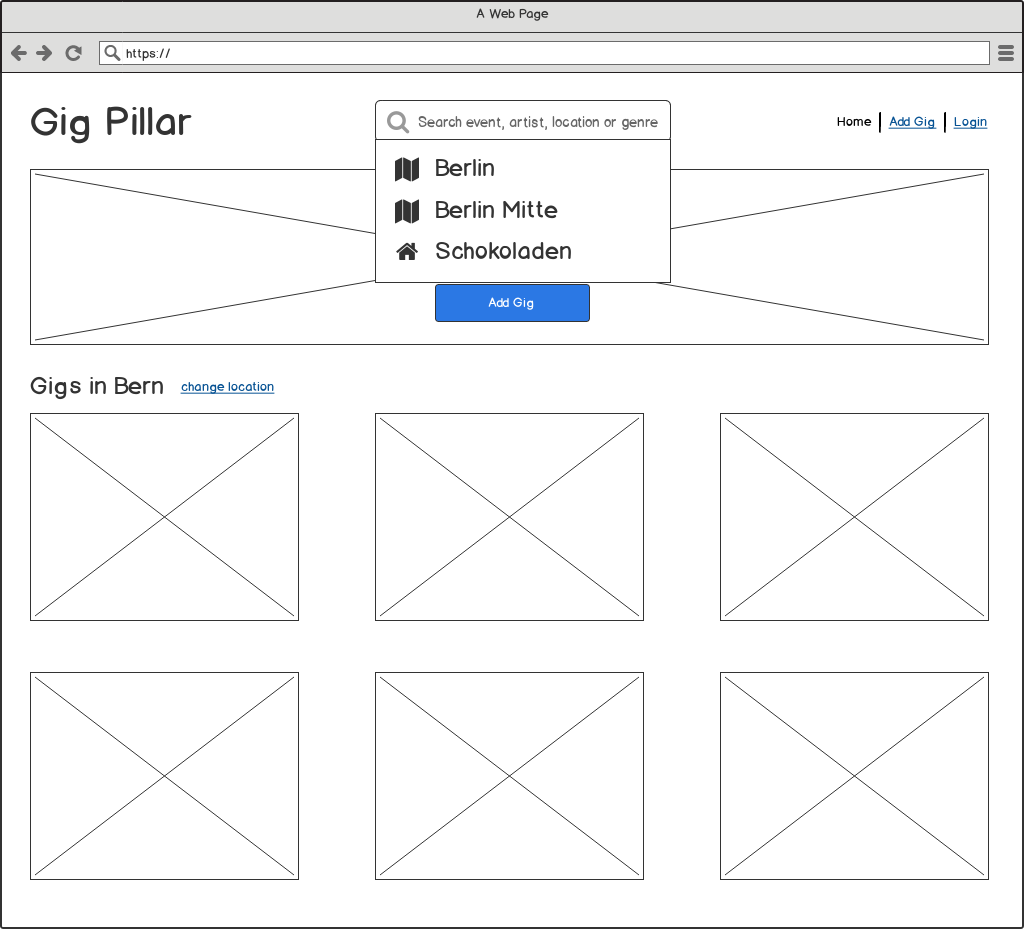
\includegraphics[width=0.95\textwidth]{mockups/homepage.png}
  \caption{Mockup: Homepage}
\end{figure}

\clearpage
\subsubsection{Suchresultate}

Auf der Suchresultate Seite sieht der Benutzer seine Suchresultate der von der
globalen Suchbox ausgelösten Suche. Die Seite bietet weitere Filter an um die
Resultate weiter einzugrenzen.\\

\noindent
Folgende Filter stehen den Benutzern zur Verfügung:

% TODO: This diverges from our search criteria described in the previous phase.

\begin{itemize}
  \tightlist{}
  \item{} Ort
  \item{} Datum von
  \item{} Datum bis
  \item{} Musik Genre
\end{itemize}

\noindent
Das Anwählen eines Suchresultates führt den Benutzer weiter zur detaillierten
Gig Ansicht.

\begin{figure}[!htb]
  \centering
  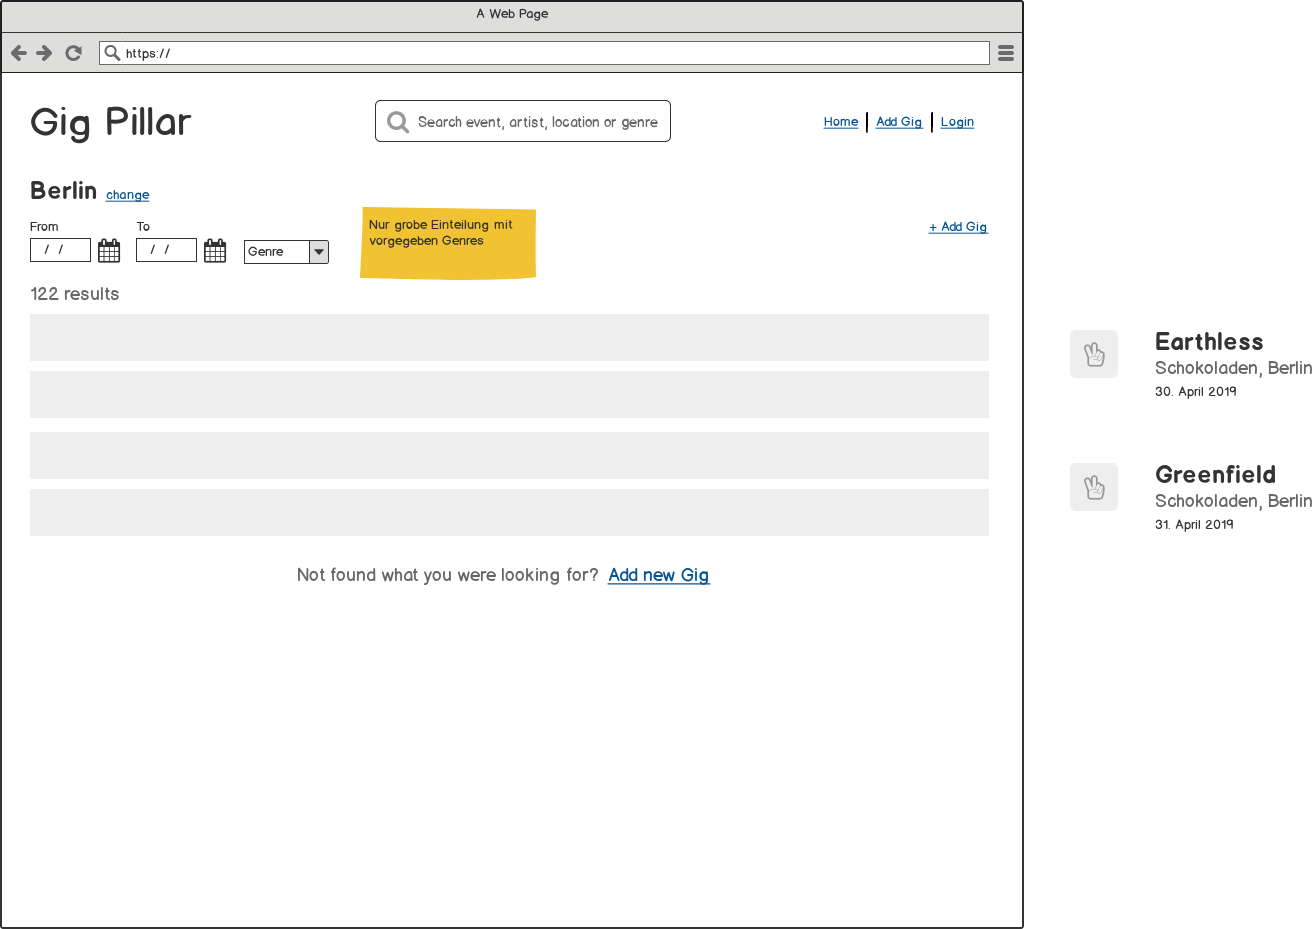
\includegraphics[width=0.95\textwidth]{mockups/search-result.png}
  \caption{Mockup: Suchresultate}
\end{figure}

\clearpage
\subsubsection{Gig Ansicht}

In der Gig Ansicht werden alle Details zu einem Event aufgelistet.

\begin{itemize}
  \tightlist{}
  \item{} Datum des Events
  \item{} Zeit wann das Event beginnt, bzw die Location die Türen öffnet
  \item{} Liste aller Künstler mit optionaler Startzeit
  \item{} Eine Beschreibung des Events
  \item{} Die Adresse der Location mit Link auf Google Maps
\end{itemize}

\noindent
Ausserdem soll es den Benutzern möglich sein, über einen «Add to my calendar»
Link das Event zu seiner Kalender-Applikation zu importieren.

\begin{figure}[!htb]
  \centering
  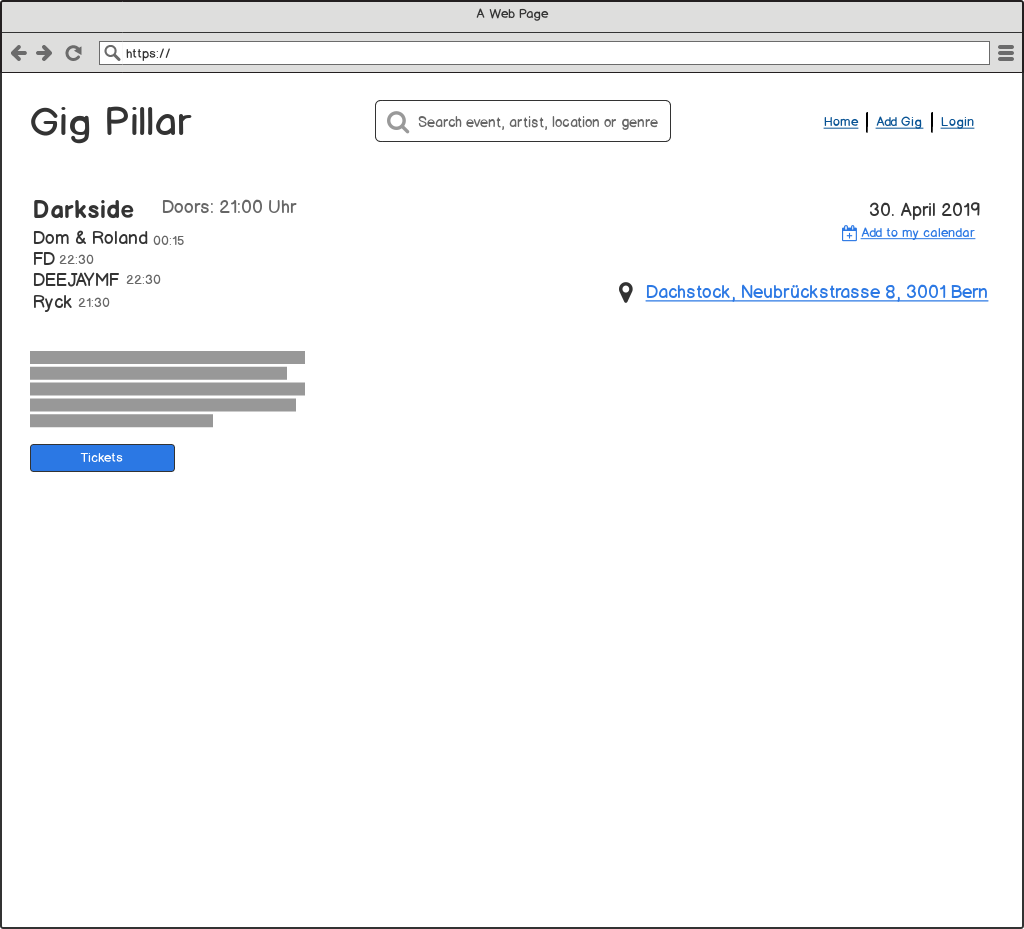
\includegraphics[width=0.95\textwidth]{mockups/event.png}
  \caption{Mockup: Gig Ansicht}
\end{figure}

\clearpage
\subsubsection{Gig erfassen}

Benutzer können Gigs erfassen.\\

\noindent
Folgende Daten sind für einen Gig zu erfassen:

\begin{itemize}
  \tightlist{}
  \item{} Name
  \item{} Bild \textit{(optional)}
  \item{} Location
  \item{} Datum
  \item{} Zeit
  \item{} Eine Liste von Artists mit optionaler Startzeit
  \item{} Beschreibung
  \item{} Link zum Ticketvertreiber
\end{itemize}

\begin{figure}[!htb]
  \centering
  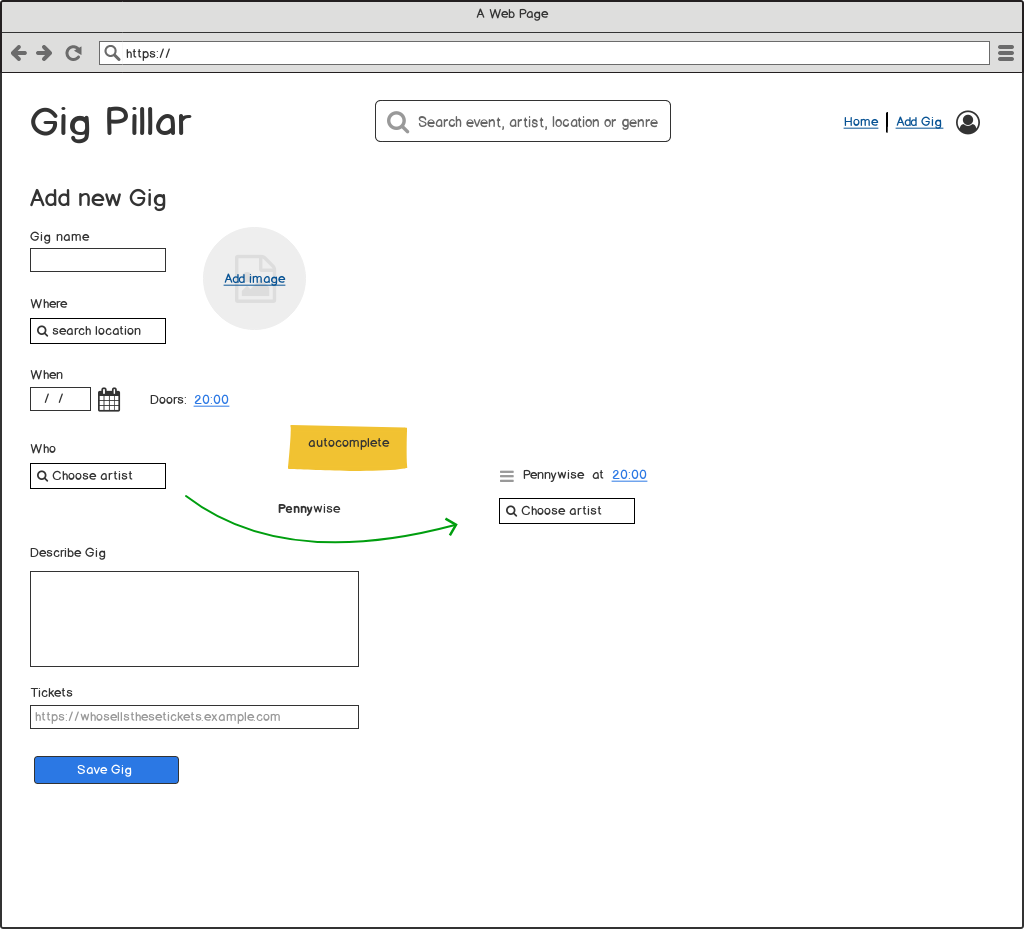
\includegraphics[width=0.95\textwidth]{mockups/add-gig.png}
  \caption{Mockup: Gig erfassen}
\end{figure}

\clearpage
\subsubsection{Benutzerprofil}

Benutzer können ihr eigenes Profil verwalten und folgende Tätigkeiten
verrichten:

\begin{itemize}
  \tightlist{}
  \item{} Anzeigename ändern
  \item{} E-Mail Adresse ändern \textit{(mit E-Mail Bestätigung)}
  \item{} Passwort ändern \textit{(muss vorher altes Passwort bestätigen)}
  \item{} Account löschen \textit{(muss doppelt bestätigt werden!)}
\end{itemize}

\begin{figure}[!htb]
  \centering
  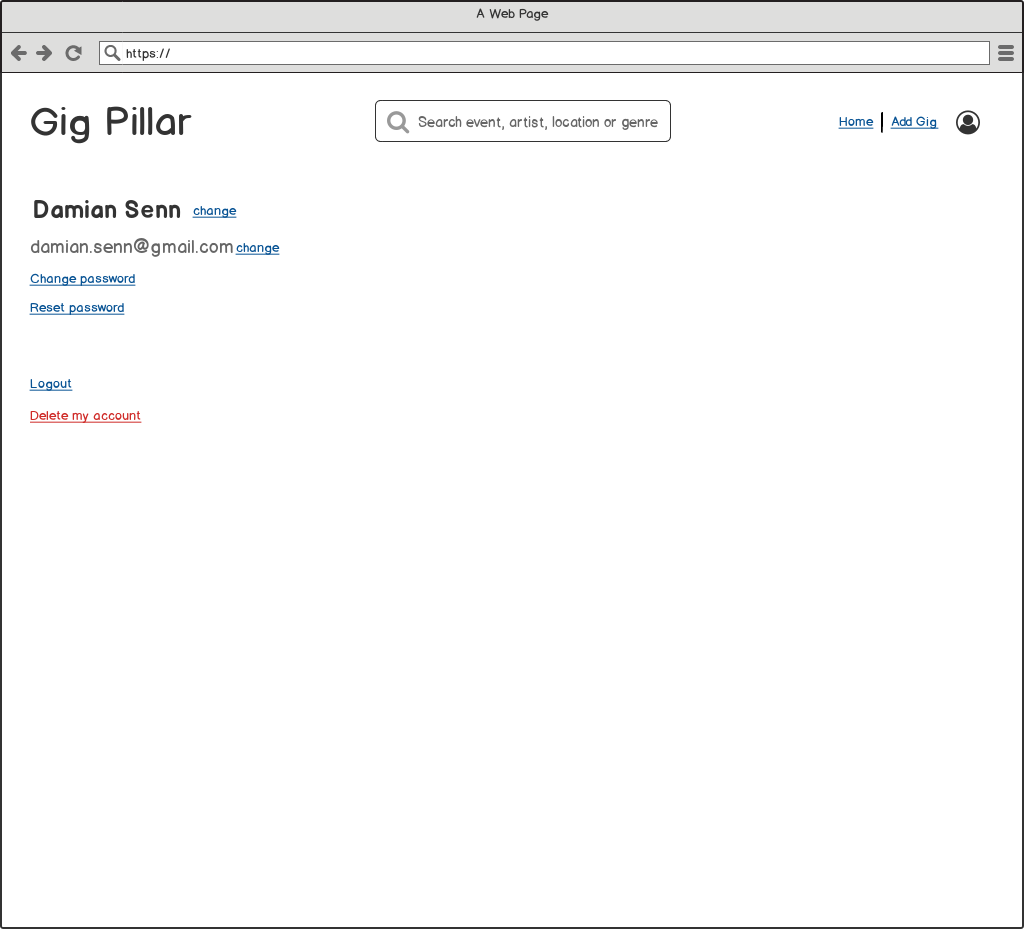
\includegraphics[width=0.95\textwidth]{mockups/profile.png}
  \caption{Mockup: Benutzerprofil}
\end{figure}

\clearpage
\subsection{Genre Filter}\label{genrefilter}

Der Genre Filter soll folgende Werte zur Verfügung stellen.

\begin{itemize}
  \item{} Alternative
  \item{} Blues
  \item{} Classical
  \item{} EDM
  \item{} Hip-Hop
  \item{} Jazz
  \item{} Metal
  \item{} Pop
  \item{} Punk
  \item{} Reggae
  \item{} Rock
\end{itemize}

\clearpage
\section{Softwarekonzept}\label{softwarekonzept}
\subsection{Datenfluss}\label{datenfluss}

\subsubsection{Homepage}\label{datenfluss-homepage}

Die Homepage zeigt den Besuchern Gigs in ihrer Nähe an, dazu muss über eine
GeoIP API die IP-Adresse des Besuchers auf ein Land zurückverfolgt werden.
Dazu wird beim ersten Besuch die GeoIP API abgefragt und das Land des Benutzers
in eine Session geschrieben. Bei weiteren Aufrufen wird das Land direkt aus der
Session bezogen.

%GigPillarWeb
%GigPillarWeb_Session
%GigPillar
%GeoIp
%
%Response = GigPillarWeb./ {
%  if (hasSession) {
%    location = GigPillarWeb_Session.getLocation()
%  } else {
%    location = GigPillarWeb_Session.createSession() {
%      location = GeoIp.getLocation(ip)
%    }
%  }
%
%  Events = GigPillar.getUpcomingEvents(location)
%}

\begin{figure}[!htb]
  \centering
  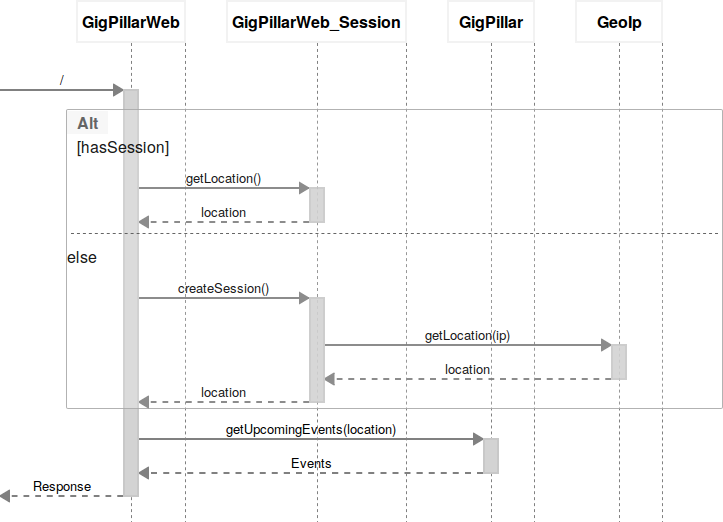
\includegraphics[width=0.95\textwidth]{konzept/datenfluss-homepage.png}
  \caption{Datenfluss: Homepage}
\end{figure}

\clearpage
\subsubsection{Suchfeld}\label{datenfluss-suchfeld}

Das globale Suchfeld hat eine Autocompletion, welche Daten direkt von
der GigPillar Applikation bezieht. Die Daten für Städtenamen wird jedoch von
einer externen Datenquelle, z.B. Google Maps, bezogen.

%GigPillarWeb
%GigPillar
%GoogleMaps
%
%Response = GigPillarWeb./searchCompletion {
%  Cities = GoogleMaps.searchCities(searchParameters)
%  Locations = GigPillar.searchLocations(searchParameters)
%  Genres = GigPillar.searchGenres(searchParameters)
%  Artists = GigPillar.searchArtists(searchParameters)
%  Events = GigPillar.searchEvents(searchParameters)
%}

\begin{figure}[!htb]
  \centering
  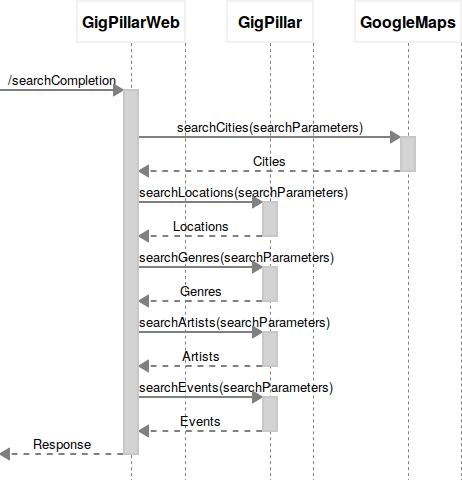
\includegraphics[width=0.95\textwidth]{konzept/datenfluss-suchfeld.png}
  \caption{Datenfluss: Suchfeld}
\end{figure}

\clearpage
\subsubsection{Gig erstellen - Locationfeld}\label{datenfluss-gig-erstellen-locationfeld}

Beim Erstellen eines neuen Gigs, muss eine Location zugewiesen werden. Die
Locations werden über die bereits in GigPillar erfassten Locations sowie über
eine externe Datenquelle, wie z.B. Google Maps, bezogen.

%GigPillarWeb
%GigPillar
%GoogleMaps
%
%Response = GigPillarWeb./locationCompletion {
%  Locations = GigPillar.searchLocations(searchParameters) {
%    Locations = searchLocations(searchParameters)
%    Locations = GoogleMaps.searchLocations(searchParameters)
%  }
%}

\begin{figure}[!htb]
  \centering
  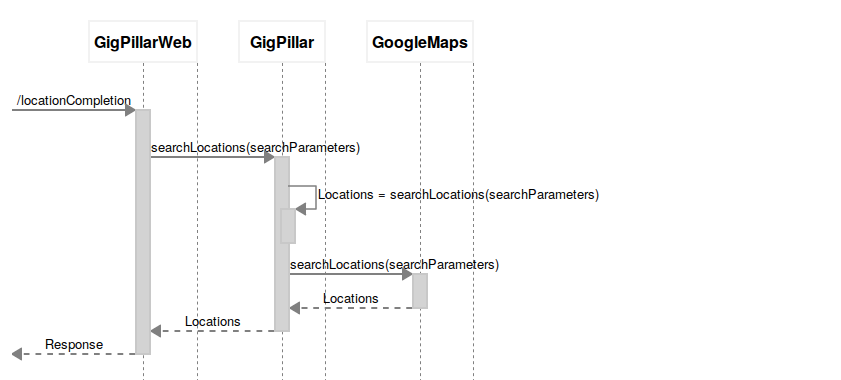
\includegraphics[width=0.95\textwidth]{konzept/datenfluss-locationfeld.png}
  \caption{Datenfluss: Gig erstellen - Locationfeld}
\end{figure}

%TODO:
%\clearpage
%\subsubsection{Gig erstellen - Artistfeld}

% Autocomplete, +lastfm?

%TODO:
%\clearpage
%\subsubsection{Gig erstellen}\label{datenfluss-gigerstellen}

% Optional FB-Event erstellen

\clearpage
\subsubsection{Passwort-Reset}\label{datenfluss-passwort-reset}

Falls ein Benutzer sein Passwort vergessen hat, kann dieser ein neues Passwort
über die Passwort-Reset Funktion setzen. Beim Auslösen eines Passwort-Resets,
wird dem Benutzer ein E-Mail mit einem Link zugeschickt.
Der Passwort-Reset-Link führt den Benutzer auf ein Formular auf welchem er/sie
die Möglichkeit hat, ein neues Passwort zu setzen.

%GigPillarWeb
%GigPillar
%UserEmailClient
%
%Response = GigPillarWeb./passwordReset {
%  GigPillar.sendPasswordResetEmail(email) {
%    GigPillar->UserEmailClient:SMTP
%  }
%}
%
%Redirect = UserEmailClient.clickPasswordResetLink {
%  Response = GigPillarWeb./passwordRestToken
%}
%
%Response = GigPillarWeb./setPassword {
%  GigPillar.setUserPassword(currentUser, password)
%}

\begin{figure}[!htb]
  \centering
  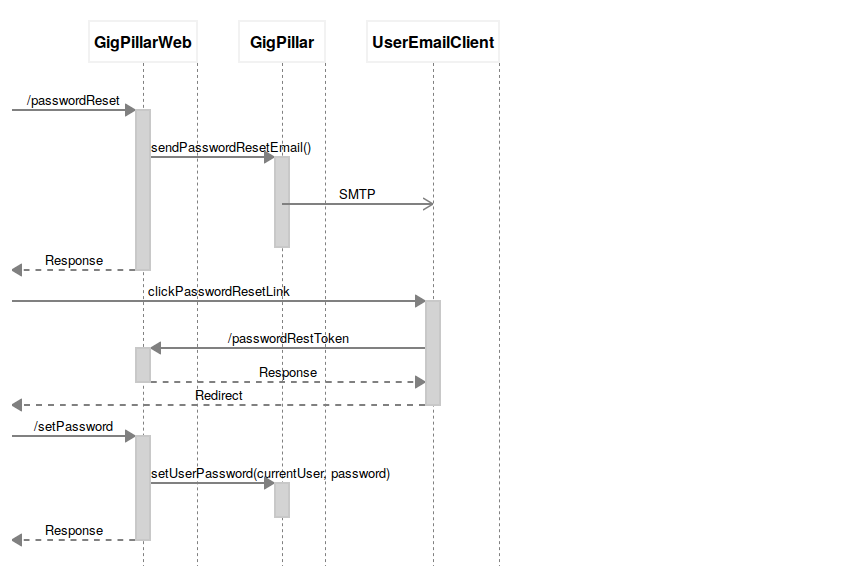
\includegraphics[width=0.95\textwidth]{konzept/datenfluss-passwort-reset.png}
  \caption{Datenfluss: Passwort-Reset}
\end{figure}

\clearpage
\subsection{Datenbankstruktur}\label{datenbankstruktur}

\begin{figure}[!htb]
  \centering
  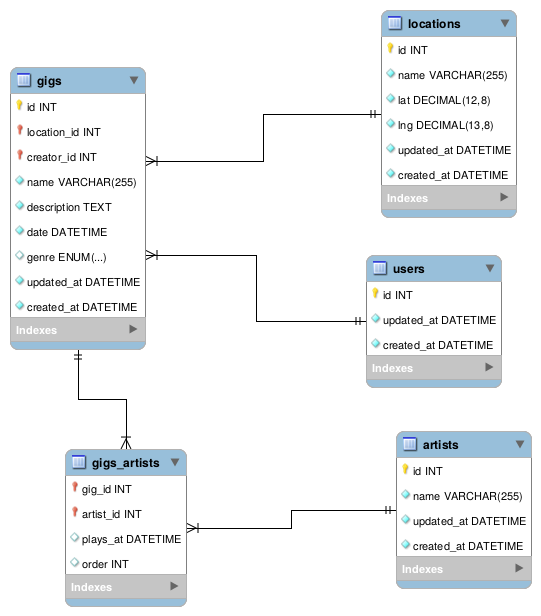
\includegraphics[width=0.95\textwidth]{konzept/erd.png}
  \caption{Konzept: Entity Relationship Diagram}
\end{figure}

% Genre on Gig, why?

\clearpage
\section{Testkonzept}\label{testkonzept}

\subsection{Unit-Tests}\label{unittests}

Der Applikationscode soll mit Unit-Tests getestet werden und mindestens eine
Abdeckung von 80\% des Codes erfüllen.

Unit-Tests testen einzelne Funktionen, d.h. hier sind Aufrufe über HTTP, wie
sie durch den Browser ausgelöst würden, oder Datenbankabfragen ausgeschlossen.

\subsection{Integration-Tests}\label{integrationtests}

HTTP Requests sowie Datenabfragen sollen über Integration-Tests abgedeckt
werden. In den Integration-Tests wird vor allem Business-Logik wie z.B.
Validierungen von Daten getestet.

\subsection{Browser-Tests}\label{browsertests}

Mit der in der Studie evaluierten Testing Library «Wallaby» sollen die
gängigsten Benutzer Use-Cases getestet werden.

\subsection{Visual-Tests}\label{visualtests}

Es soll für jede Ansicht während den Tests mindestens ein Screenshot für
\href{https://percy.io/}{percy.io} erstellt werden.

\clearpage
\subsection{Akzeptanztests}\label{akzeptanztests}

Die Akzeptanztest sind vom Projektleiter vor Abschluss der Realisierung
durchzuführen. Der Umfang der Akzeptanztests basiert auf den Kriterien die im
Anforderungskatalog definiert wurden.

Technische Kritierien wie die Indexierbarkeit wurden in den Akzeptanztests
bewusst ausgelassen, die Tests sollen möglichst unabhängig vom System
durchführbar sein.

\newcounter{acceptancetest}

\NewDocumentCommand{\acceptancetest}{
  O{}
  O{}
  O{\tabularnewline\tabularnewline}
  O{\tabularnewline\tabularnewline\tabularnewline\tabularnewline}
  m
  m
}{
  \stepcounter{acceptancetest}
  \begin{longtable}[]{@{}l|p{6cm}p{4cm}@{}}
    \toprule
    \textbf{Test \ifnum\value{acceptancetest}<10 0\fi\arabic{acceptancetest}} & \textbf{Tester:} #1                         & \textbf{Datum:} #2 \tabularnewline
    \midrule
    \textbf{Kriterium}                                                        & \multicolumn{2}{p{10cm}}{#5}\tabularnewline
    \textbf{Erwartetes Ergebnis}                                              & \multicolumn{2}{p{10cm}}{#6}\tabularnewline
    \midrule
    \textbf{Testergebnis}                                                     & #3\tabularnewline
    \midrule
    \textbf{Fehlerbeschreibung}                                               & #4\tabularnewline
    \bottomrule
    \caption{Akzeptanztest \ifnum\value{acceptancetest}<10 0\fi\arabic{acceptancetest}}
  \end{longtable}
}

\acceptancetest
{Es ist möglich nach Konzerten in einem bestimmten Ort zu suchen.}
{Nach auswählen von «Berlin» in der Suche, werden nur noch Konzerte in Berlin aufgelistet.}

\acceptancetest
{Es ist möglich eine Suche weiter nach Genre einzuschränken.}
{Nach auswählen von «Rock» in einem Suchresultat, werden nur noch Rock-Konzerte aufgelistet.}

\clearpage

\acceptancetest
{Responsive - Homepage}
{Sieht auf Desktop, Tablet und Mobile gut aus und stellt jeweils alle relevanten Daten dar.}

\acceptancetest
{Browserkompatibilität - Homepage}
{Funktioniert in den unterstützten Browsern.}

\clearpage

\acceptancetest
{Responsive - Suche}
{Sieht auf Desktop, Tablet und Mobile gut aus und stellt jeweils alle relevanten Daten dar.}

\acceptancetest
{Browserkompatibilität - Suche}
{Funktioniert in den unterstützten Browsern.}

\clearpage

\acceptancetest
{Responsive - Gig Ansicht}
{Sieht auf Desktop, Tablet und Mobile gut aus und stellt jeweils alle relevanten Daten dar.}

\acceptancetest
{Browserkompatibilität - Gig Ansicht}
{Funktioniert in den unterstützten Browsern.}

\clearpage

\acceptancetest
{Responsive - Login}
{Sieht auf Desktop, Tablet und Mobile gut aus und stellt jeweils alle relevanten Daten dar.}

\acceptancetest
{Browserkompatibilität - Login}
{Funktioniert in den unterstützten Browsern.}

\clearpage

\acceptancetest
{Responsive - Registrierung}
{Sieht auf Desktop, Tablet und Mobile gut aus und stellt jeweils alle relevanten Daten dar.}

\acceptancetest
{Browserkompatibilität - Registrierung}
{Funktioniert in den unterstützten Browsern.}

\clearpage

\acceptancetest
{Responsive - Gig erfassen}
{Sieht auf Desktop, Tablet und Mobile gut aus und stellt jeweils alle relevanten Daten dar.}

\acceptancetest
{Browserkompatibilität - Gig erfassen}
{Funktioniert in den unterstützten Browsern.}

\clearpage

\acceptancetest
{Gig erfassen}
{Folgende Daten können erfasst werden:
  \begin{itemize}
    \tightlist{}
    \item{} Name
    \item{} Bild \textit{(optional)}
    \item{} Location
    \item{} Datum
    \item{} Zeit \textit{(optional)}
    \item{} Künstler mit optionaler Start-Zeit
    \item{} Beschreibung
    \item{} Link zum Ticketvertreiber \textit{(optional)}
  \end{itemize}}

\acceptancetest
{Neue Gigs tauchen in der Suche auf.}
{Der neu erstellte Gig taucht in der Suche auf.}

\clearpage

\acceptancetest
{Responsive - Benutzerprofil}
{Sieht auf Desktop, Tablet und Mobile gut aus und stellt jeweils alle relevanten Daten dar.}

\acceptancetest
{Browserkompatibilität - Benutzerprofil}
{Funktioniert in den unterstützten Browsern.}

\clearpage

\acceptancetest
{Responsive - Passwort-Reset}
{Sieht auf Desktop, Tablet und Mobile gut aus und stellt jeweils alle relevanten Daten dar.}

\acceptancetest
{Browserkompatibilität - Passwort-Reset}
{Funktioniert in den unterstützten Browsern.}

\clearpage

\acceptancetest
{Security - Suche}
{Das Suchfeld ist resistent gegen XSS und SQL-Injection}

\acceptancetest
{Security - Login}
{Das Login ist resistent gegen XSS und SQL-Injection}

\clearpage

\acceptancetest
{Security - Benutzerprofil}
{Das Benutzerprofil ist resistent gegen XSS und SQL-Injection}

\acceptancetest
{Security - Gig erfassen}
{Das Gig erfassen Formular ist resistent gegen XSS und SQL-Injection}

\clearpage
\section{Fazit}\label{konzept-fazit}

\subsection{Probleme}

% Abweichung "Filter-System" in Suche?
% Genres? In Gig oder Artist?
% Einfachheit von Erfassen eines Gigs, Dateninkonsistenzen?

\subsection{Machbarkeit}

% Erstellung Location / Artist vorerst auslassen?
% Location vorerst auf Google Maps limitieren?
% Google Maps API?

\subsection{Wirtschaftlichkeit}

% Änderung an Aufwand?

\subsection{Erweiterbarkeit}

% FB Events etc?

\subsection{Projektplan}
